\chapter{Machine Learning Models}
Machine learning is a scientific discipline focused on the development of
algorithms based on learning from examples. This idea has become central to the
design of search engines, robots systems and forecasts applications that
process large data sets. Usually machines designed to forecast financial time
series requires long training period and therefore they are not suitable to be updated
with stream data. Online machine learning techniques tackle this problem by updating the model with new
data or by computing a new model using less data so they can give a response in a
short period of time.

\vspace{0.5cm} 

\section{Introduction}
Machine Learning (ML) studies computer algorithms for learning
something such as to complete a task, to make accurate predictions or to behave intelligently. The learning is always based on samples and the objective is about to do better in the future based on the past experiences in an automatic way. ML is a sub-area of artificial intelligence and broadly intersects with other fields such as statistics, mathematics, physics and computer science. 
There are many examples of machine learning problems: time series forecasting, image processing, face detection, spam filtering, weather prediction, search engines, among many others.

ML models are often more accurate than what can be created through direct programming. The reason for this is that ML models are data driven and are able to examine large amounts of data.

There are three types of ML classified depending on the nature of the learning input or output available to a learning system:

\begin{description}
\item[Supervised learning]  the input data is a tuple which contains the example input and its desired outputs (also called labels). The list of tuples is called the training set. The concept of supervised learning comes from the supervisor, acting as a teacher in the learning process. The goal is to learn a general rule that maps inputs to outputs optimising a target function. There are two related problem types in supervised learning: classification and regression problems \cite{bishop2006}. Its two mainstream approaches are: support vector machines (SVMs) \cite{vapnik1998} and ensemble learning \cite{breiman1998}. Furthermore, supervised learning can be categorised into offline or batch learning and online learning (see section \ref{sec:onoffline}). 
\item[Unsupervised learning] also known as clustering \cite{ben2005}. In this type of learning no labels are given and the system has to find a structure on its own, discovering hidden patterns in data.
\item[Reinforcement learning] is the problem faced by an agent that must learn 
through trial-and-error interactions with a dynamic environment. It is based on programming agents by reward and punishment without the need to specify how the task is to be achieved \cite{sutton1998}.
\end{description}


\section{Statistical learning theory} \label{sec:mltheory}

All ML problems can be viewed as optimisation problems. The ML core task is to define a learning criterion, i.e the function to be optimised. 

Supervised learning is most popular and most commonly used in modelling financial problems and the assessments of this method and their results in practice are fairly good. Therefore, in this thesis we will adhere to this trend and we will use supervised learning.

Supervised learning consists in finding a learning function $f: X \rightarrow Y$ which models a set of examples, called training set $S$, which have been drawn randomly and independently according to a unknown joint distribution function $p(x,y)$ on $X \times Y$:


$$
S = \{ (x_k,y_k)\in X\times Y : k=1,...,n \}
$$

\noindent where $X \subseteq \mathbb{R}^m$ and $Y = \mathbb{R}$ in case of regression problems and $Y = \{1,-1\}$  if it is a classification problem. 

A learning algorithm $\mathcal{A}$ takes as input a data set $S \in \mathscr{T}=\mathscr{P}(X\times Y)$ and selects from $\mathcal{H}$ a function $f$ such that $f(x)\approx y $ in a predictive way:

\begin{eqnarray*}
\mathcal{A}: \mathscr{T} &\rightarrow & \mathcal{H} \\
S &\rightarrow &\mathcal{A}(S) = f
\end{eqnarray*}

\noindent where $\mathcal{H}$ is called the {\em hypothesis space}, is the space of functions that the algorithm is allowed to search. The selection of $f$ is based on the minimization of the expected error of the loss function $V(f(x),y)$ defined as:

\begin{eqnarray*}
 V(f(\cdot),\cdot): X\times Y &\rightarrow & Y \\
  (x, y) &\rightarrow &V(f(x),y)
\end{eqnarray*}

\noindent $V(f(x),y)$ denote the price paid for mistakes. Therefore, $V(f(x),y)=0$ if $f(x)=y$.

Given a function $f$ a loss function $V$ and a probability distribution $p$ over $X \times Y$, the expected error of $f$ is:

\begin{equation}
\label{eq:expetedrisk}
E[V(f(\cdot),\cdot)] = \int_{X\times Y} V(f(x),y)\;dp(x,y)\,,
\end{equation}


For regression, the most common loss function is square loss or L2 loss function:
\begin{equation}
\label{eq:l2loss}
V(f(x),y) = (f(x)-y)^2
\end{equation}
\noindent another option is the L1 loss
\begin{equation}
\label{eq:l1loss}
V(f(x),y) = |f(x)-y| \, .
\end{equation}
\noindent the choice of loss function here gives rise to several well-known learning algorithms such as regularised least squares and support vector machines. %verificar esto

Since the true distribution is unknown and only training samples are available, the objective is to estimate a function $\hat{f}$ through empirical risk (training error) minimisation (ERM): 

\begin{equation} 
\label{eq:erm}
R_{\text{emp}}[f] = \frac{1}{n} \sum_{i=1}^n V(f(x_i),y_i)
\end{equation}

The ERM is a Riemann sum approximation of the expected error of $f$ shown in equation \ref{eq:expetedrisk}, where $dp(x,y) \approx 1/n$.

\subsection{Learning algorithms}
In all learning algorithms that are trained from example data, there is a tradeoff \cite{dietterich2003} between three factors:
\begin{description}
\item[Complexity of the hypothesis class] for best generalisation, we should adjust the complexity of the learner model $\hat{f}$ to the complexity of the data $f$. The complexity of a learning problem mostly depends on the number of training examples and the size of the searched hypothesis space. In polynomial regression, the complexity parameter is the order of the fitted polynomial, and therefore we need to find a way to choose the best order that minimises the generalisation error, that is, tune the complexity of the model to best fit the complexity of the function inherent in the data.
\item[Generalisation accuracy on new examples] is the capability of the algorithm to generate the right output for an input instance outside the training set. It is measured by the expected risk (equation \ref{eq:expetedrisk}).
\item[The amount of training data]  in most cases, generalisation accuracy increases as the amount of training data increases.
\end{description}

Very complex models will fit the training data better (low bias) but it could overfit it and generalise poorly (high variance), this is also called the bias-variance tradeoff.  Generalisation accuracy can sometimes be improved with more training data. The figure \ref{fig:tradeoff} illustrates how generalisation accuracy depends on the complexity of the model and the amount of training data.

\begin{figure}[!h]
  \centering
  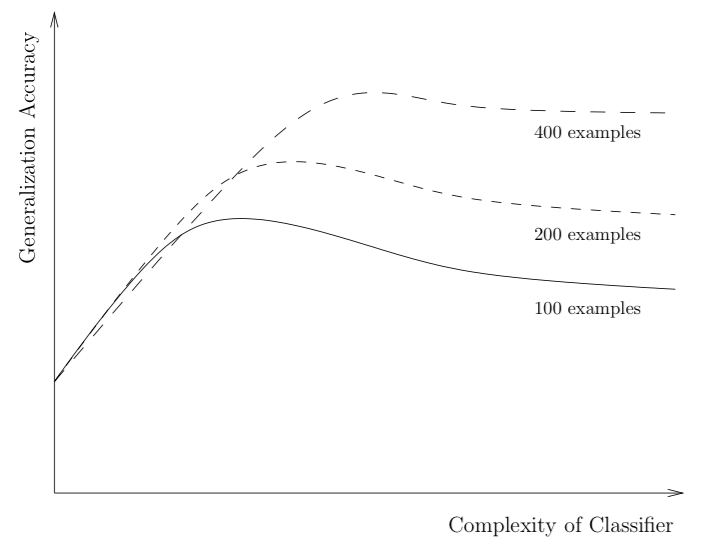
\includegraphics[width=0.8\textwidth]{img/3tradeoff}
  \caption{Tradeoff in empirical learning from \cite{dietterich2003}. The generalization accuracy is not affected by the amount of examples for low complex classifiers. However, for some more complex classifiers, the number of examples improves the generalization accuracy. The key is to find the best generalization accuracy and the lowest complex classifier as possible. }
  \label{fig:tradeoff}
\end{figure}

\subsection{The bias-variance tradeoff} \label{sec:biasvar}

Models learning error can be split into two main components: error due to bias and error due to variance. Bias measures how far off in general these models' predictions are from the correct value. Variance is taken as the variability of a model prediction for a given data point.

If we have a learning model $\hat{f}$, its expected generalisation error on an unseen or testing sample $x$ can be decomposed as follows:

\begin{align}
\label{eq:bvtrade}
\mathrm{E}\Big[\big(y - \hat{f}(x)\big)^2\Big]
 & = \mathrm{Bias}(\hat{f}(x))^2 + \mathrm{Var}(\hat{f}(x)) + \sigma^2
\end{align}
\noindent where:
\begin{align*}
 \mathrm{Bias}(\hat{f}(x)) &= \mathrm{E}\big[\hat{f}(x)\big] - f(x) \\
 \mathrm{Var}(\hat{f}(x)) &= \mathrm{E}\Big[ \big( \hat{f}(x) - \mathrm{E}[\hat{f}(x)] \big)^2 \Big] 
\end{align*}


\textbf{Demo}\quad

\begin{eqnarray*}
E[(y-\hat{f}(\mathbf{x}))^2] & =&
E[(y-f(\mathbf{x})+f(\mathbf{x})-\hat{f}(\mathbf{x}))^2] \\
&=& E[(B-f(\mathbf{x}))^2] +
E[(f(\mathbf{x})-\hat{f}(\mathbf{x}))^2] + \dots \\
& &
2\cancelto{0}{E[y-f(\mathbf{x})]}E[f(\mathbf{x})-\hat{f}(\mathbf{x})] \\
&=& \sigma^2 + MSE(\hat{f}(\mathbf{x}))
\end{eqnarray*}

\noindent where 

\begin{eqnarray*}
    MSE(\hat{f}(\mathbf{x})) &=&
    E[f(\mathbf{x})-\hat{f}(\mathbf{x}))]^2 \\
    &=& E[f(\mathbf{x})-E[\hat{f}(\mathbf{x})] +
    E[\hat{f}(\mathbf{x})]-\hat{f}(\mathbf{x}))]^2 \\
    &=&  E[(f(\mathbf{x})-E[\hat{f}(\mathbf{x})])^2] +
      E[(\hat{f}(\mathbf{x})-E[\hat{f}(\mathbf{x})])^2] + \dots\\
    & & E[(f(\mathbf{x})-E[\hat{f}(\mathbf{x})])] 
    \cancelto{0}{E[(\hat{f}(\mathbf{x})-E[\hat{f}(\mathbf{x})])]} \\
    &=& Bias(\hat{f}(\mathbf{x}))^2 + Var(\hat{f}(\mathbf{x}))
\end{eqnarray*}

$\blacksquare$

Bias is introduced by the model selection. Therefore the model building process is repeated (through resampling) and substantially different averages of prediction values are obtained, bias will be high. The error due to variance is the amount by which the prediction, over one training set, differs from the expected predicted value, over all the training sets. Variance measures how inconsistent are the predictions from one another, over different training sets, not whether they are accurate or not.

This generalisation error is unknown, but it can be estimated using a training sample, a testing sample or by estimating the model complexity. Figure \ref{fig:traintesterror} shows prediction error for training and testing sample.  In general, in the training sample prediction error is decreasing with more complex models but it overfit the data and it is not a good model for the test data. Figure \ref{fig:bvtradeoff} shows how testing error can be decomposed into bias and variance components. The best model will be the one has a balance between bias and variance.

\begin{figure}[!h]
  \centering
  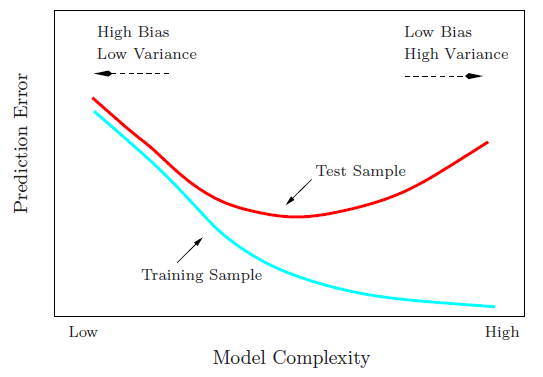
\includegraphics[width=0.8\textwidth]{img/model_complexity}
  \caption{Training and test error}
  \label{fig:traintesterror}
\end{figure}


The objective is to simultaneously reduce bias and variance as much as possible in order to obtain as accurate model as is feasible.  However, there is a tradeoff to be made when selecting models. Models that exhibit small variance and high bias underfit the truth target.  Models that exhibit high variance and low bias overfit the truth target.

This bias-variance tradeoff is the reason why in order to obtain the best model, data is usually broken in three subsets: training set, validation set and testing set. Training set is used to determine the model, validation set is used to estimate the generalisation error and finally testing set is used to estimate the accuracy of the model. Usually the partition is 50\% for training set, 25\% for validation and 25\% for testing purposes. This procedure can be extended to a Cross Validation (CV) procedure \cite{geisser1975}, usually used when the amount of data is limited. Various splitting strategies lead to various CV estimates. In K-fold cross-validation the training data is divided randomly into K distinct subsets, then the network is trained using K-1 subsets, and tested on the remaining subset. The process of training and testing is then repeated for each of the K possible choices of the subset omitted from the training. The average performance on the K omitted subsets is then our estimate of the generalisation performance.

\begin{figure}[!h]
  \centering
  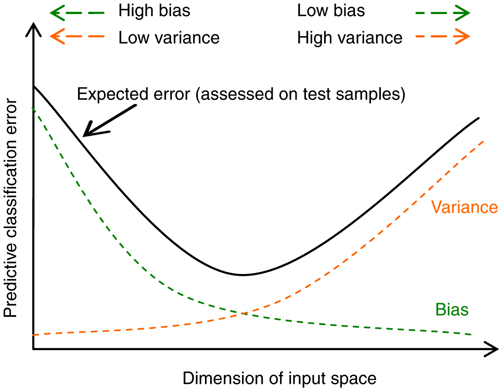
\includegraphics[width=0.8\textwidth]{img/biasvariancetradeoff}
  \caption{Bias variance tradeoff}
  \label{fig:bvtradeoff}
\end{figure}

Another way to control the complexity of the model is to include in the optimisation function not only the generalisation error but a penalisation of high complex models. 


\subsection{Regularization}

Regularization can be understood using two contexts: learning theory (probabilistic) and inverse problems (deterministic). In the context of learning, regularization refers to techniques allowing to avoid over-fitting and the desire property of the selected estimator is to perform well on new data (to generalize), e.g. regularized least squares. In the context of inverse problems, regularization objective is to stabilise, with respect to noise, a possibly ill-conditioned matrix inversion problem e.g spectral cut-off and Tikhonov regularization or ridge regression (RR)\cite{ tikhonov1977}.

In particular, it is well known that regularization schemes such as RR or Tikhonov regularization can be effectively used in the context of learning \cite{vito2005}.

Tikhonov introduced a regularisation which ensures well-posedness and generalisation of ERM, i.e prevents overfit, by constraining the hypothesis space $\mathcal{H}$ usually called regularised ERM or Tikhonov regularisation.

Tikhonov regularisation minimised over the hypothesis space $\mathcal{H}$ for a fixed positive parameter $\lambda$ the following:

\begin{equation} 
\label{eq:rerm}
R_{\text{emp}}[f] = \frac{1}{n} \sum_{i=1}^n V(f(x),y) + \lambda \mathcal{R}(f)
\end{equation}

\noindent where $\mathcal{R}(f)$ is the regulariser, a penalisation on $f$.

\subsection{Ridge Regression}



One example of regularisation in linear models is Ridge Regression (RR), which is a regularised least squares method.
The least squares (LS) method is a well known way to solve a regression
problem. 
LS method consists of minimising the sum of squared errors:

\begin{eqnarray*}
\label{eq:lsm}
 J(\mathbf{X}) =& \displaystyle \sum_{t=1}^N (f(\mathbf{x}_t)-y_t)^2 \\
 =&\displaystyle \sum_{t=1}^N (\mathbf{\mathbf{X}}^\top {\mathbf{x}}_t-y_t)^2 \\
 =& \| \mathbf{A}\mathbf{\mathbf{X}} - \mathbf{Y} \|_2^2 
\end{eqnarray*}

\noindent which is equivalent to find a solution to 
\begin{equation}
\label{eq:regproblem}
\underset{m \times n}{\mathbf{A}} \enskip \underset{n \times
l}{\mathbf{\mathbf{X}}} = \underset{m \times l}{\mathbf{Y}}
\end{equation}

The optimal solution for $\mathbf{\mathbf{X}}$ is:
\begin{equation}
\label{eq:MP}
\mathbf{\mathbf{X}}= \mathbf{A}^+ \mathbf{Y}
\end{equation}

\noindent where $\mathbf{A}^+$ is the Moore-Penrose pseudo-inverse
which can be written as follows: 

\begin{equation}
\label{eq:pseudoinverse}
\mathbf{A}^+= (\mathbf{A}^\top \mathbf{A})^{-1}\mathbf{A}^\top \, .
\end{equation}

\textbf{Demo}\quad

To solve equation~(\ref{eq:pseudoinverse}) is equivalent to solve the following
optimisation problem:


\begin{equation}
\label{eq:RRproblem2}
\underset{\mathbf{X}(\lambda)}{\text{min}} \quad \|
\mathbf{C}\mathbf{\mathbf{X}} - \mathbf{F} \|_2^2
\end{equation}

\noindent where

\begin{equation*}
	\mathbf{C}=
	\begin{bmatrix} \quad &\mathbf{A}& \quad \\ \hdashline \quad
& \sqrt\lambda\mathbb{I}&\quad  
\end{bmatrix} 
\quad \text{and} \quad
	\mathbf{F}=\begin{bmatrix} \quad &\mathbf{Y}& \quad \\ \hdashline \quad
& \mathbf{0}&\quad  \end{bmatrix} \, .
\end{equation*}

Applying equation~(\ref{eq:MP}) and considering that $\mathbf{C}^\top
\mathbf{C} = \mathbf{A}^\top \mathbf{A} + \lambda \mathbb{I}$ and 
$\mathbf{C}^\top \mathbf{F}=\mathbf{A}^\top \mathbf{Y} $ we have:

\begin{eqnarray*}
\mathbf{X}(\lambda)&=&(\mathbf{C}^\top
\mathbf{C})^{-1}\mathbf{C}^\top \mathbf{F} \\
&=& (\mathbf{A}^\top \mathbf{A} + \lambda \mathbb{I})^{-1} \mathbf{A}^\top \mathbf{Y}
\end{eqnarray*}

$\blacksquare$


However, when $\mathbf{A}$ is not full rank, i.e
$rank(\mathbf{A})=k <  n \leq m$, $\mathbf{A}^\top \mathbf{A}$ is
always singular and equation~(\ref{eq:pseudoinverse}) cannot be used.
More generally, the pseudo-inverse is best computed using the compact
singular value decomposition (SVD) of $\mathbf{A}$:

\begin{equation}
    \label{eq:compactsvd}
    \underset{m \times n}{\mathbf{A}}=
    \underset{m \times k}{\mathbf{U_1}} \enskip
    \underset{k \times k}{\mathbf{\Sigma_1}} \enskip
    \underset{k \times n}{\mathbf{V_1}^\top}
\end{equation}

\noindent as follows

\begin{equation}
\label{eq:pseudoinversesvd}
\mathbf{A}^+ = \mathbf{V_1\Sigma_1^{-1}U_1^\top}
\end{equation}

\textbf{Demo}\quad

In the case matrix $\mathbf{A}$ is non singular, its solution is
straight forward:

\begin{equation}
\label{OLSsolution}
    \mathbf{\mathbf{X}}=\mathbf{A}^{-1}\mathbf{Y}
\end{equation}


Since the problem shown in equation~(\ref{eq:regproblem}) has not
solution, the minimum norm given by equation~(\ref{OLSsolution}) is
obtained by solving the equivalent problem:

\begin{equation*}
\label{eq:proyectorsol}
\mathbf{A \hat{\mathbf{X}} = PY} 
\end{equation*}


\noindent where $\mathbf{P=U_1 U_1^\top}$ is the projection onto the
Col($\mathbf{A}$). 

Since $\mathbf{V} = [\underset{(n \times k)}{\mathbf{V_1}} |
\underset{(n \times k)}{\mathbf{V_2}}]$ and $\mathbf{V_1^\top V_2 =
0}$ we can express $\mathbf{\hat{\mathbf{X}}} = \mathbf{V_1 \mathbf{X}_1 + V_2 \mathbf{X}_2}$
with $\mathbf{\mathbf{X}_2=0}$ because $\mathbf{\hat{\mathbf{X}}}$ lives in the
$\text{Row}(\mathbf{A})$ given by $\mathbf{V_1}$, so we have:

\begin{eqnarray*}
\mathbf{A \hat{\mathbf{X}}} &=& \mathbf{PY} \\
\mathbf{U_1 \Sigma_1 V_1^\top \hat{\mathbf{X}}} &=& \mathbf{U_1 U_1^\top Y} \\
\mathbf{ V_1^\top \hat{\mathbf{X}}} &=&  \mathbf{\Sigma_1^{-1} U_1^\top Y} \\ 
\mathbf{ V_1^\top V_1 \mathbf{X}_1} &=& \mathbf{\Sigma_1^{-1}
U_1^\top Y} \\
\mathbf{\mathbf{X}_1}&=& \mathbf{\Sigma_1^{-1} U_1^\top Y}
\end{eqnarray*}

\noindent from this result we can obtain $\mathbf{\hat{\mathbf{X}}}$ and
therefore the pseudo-inverse expression:

\begin{eqnarray*}
\mathbf{\hat{\mathbf{X}}} &=& \mathbf{V_1 \mathbf{X}_1} \\
                &=& \mathbf{V_1 \Sigma_1^{-1} U_1^\top Y} \\
\mathbf{A^+} &=& \mathbf{V_1 \Sigma_1^{-1} U_1^\top} \, .
\end{eqnarray*}

$\blacksquare$


In order to avoid the singularity of the matrix $\mathbf{A}^\top \mathbf{A}$, a regularisation term is introduced: 

\begin{equation}
\label{eq:RRproblem} 
J(\mathbf{\mathbf{X}}) =  \| \mathbf{A}\mathbf{\mathbf{X}} - \mathbf{Y} \|_2^2  + \lambda
 \| \mathbf{\mathbf{X}}\| ^2
\end{equation}

\noindent which optimal solution $\mathbf{\mathbf{X}}_*$ is well known: 

\begin{equation*}
\label{eq:optsolRR}
\mathbf{\mathbf{X}}_*=(\mathbf{A}^\top \mathbf{A}+\lambda \mathbb{I})^{-1}\mathbf{A}^\top y \, ,
\end{equation*}

\textbf{Demo}\quad

\begin{eqnarray*}
J(\mathbf{\mathbf{X}}) &=&  \| \mathbf{A}\mathbf{\mathbf{X}} - \mathbf{Y} \|_2^2  + \lambda
 \| \mathbf{\mathbf{X}}\| ^2 \\
 &=&  \sum_{t=1}^N (\mathbf{\mathbf{X}}^\top {\bf a}_t-y_t)^2 + \lambda \sum_{i=1}^p \mathbf{X}_i^2 \\
 &=& (\mathbf{X}^\top a_1-y_1)^2 + \dots + (\mathbf{X}^\top a_N-y_N)^2 + \lambda (\mathbf{X}_1^2+\dots+\mathbf{X}_p^2)
\end{eqnarray*}
\noindent taking derivatives
 \begin{eqnarray*}
 \frac{\partial J(\mathbf{\mathbf{X}})}{\partial \mathbf{X}_1}&=& 
 2(\mathbf{X}^\top \mathbf{a}_1-y_1)\mathbf{a}_{11} + \dots + 2(\mathbf{X}^\top \mathbf{a}_N-y_N)\mathbf{a}_{N1} + 2\lambda \mathbf{X}_1 \\
 &=& 2\mathbf{a}_1^\top(\mathbf{A}\mathbf{X}-\mathbf{Y}) + 2\lambda\mathbf{X}_1\\
& \vdots &\\
  \frac{\partial J(\mathbf{\mathbf{X}})}{\partial \mathbf{X}_p}&=& 
 2\mathbf{a}_p^\top(\mathbf{A}\mathbf{X}-\mathbf{Y}) + 2\lambda\mathbf{X}_p 
\end{eqnarray*}

Then we have that:
\begin{eqnarray*}
\frac{\partial J(\mathbf{\mathbf{X}})}{\partial \mathbf{X}}&=& 
 2\mathbf{A}^\top(\mathbf{A}\mathbf{X}-\mathbf{Y}) + 2\lambda\mathbf{X}
\end{eqnarray*}
Since $\frac{\partial J(\mathbf{\mathbf{X}})}{\partial \mathbf{X}}=0$ we have:
\begin{eqnarray*}
2\mathbf{A}^\top(\mathbf{A}\mathbf{X}-\mathbf{Y}) + 2\lambda\mathbf{X}&=&0 \\
\mathbf{A}^\top\mathbf{A}\mathbf{X} - \mathbf{A}^\top\mathbf{Y} + \lambda\mathbf{X} &=& 0\\
(\mathbf{A}^\top\mathbf{A}+\lambda\mathbb{I})\mathbf{X} &=&  \mathbf{A}^\top\mathbf{Y} \\
\mathbf{X} &=& (\mathbf{A}^\top\mathbf{A}+\lambda\mathbb{I})^{-1}  \mathbf{A}^\top\mathbf{Y}
\end{eqnarray*}

$\blacksquare$

\subsection{The Lambda parameter}

The additional term $\lambda \|\mathbf{\mathbf{X}}\|_2^2$ in the optimisation
problem shown in equation~(\ref{eq:RRproblem}) has two effects on the solution:
shrinks the coefficients towards zero and improves the conditioning of the
problem.

When $\mathbf{A}$ is orthonormal then $\mathbf{A}^\top \mathbf{A} =\mathbb{I}$ and there is a simple relation between the ridge estimator and the OLS estimator:
\begin{eqnarray*}
\mathbf{X}_* (\lambda) &=& (\mathbf{A}^\top \mathbf{A}+\lambda \mathbb{I})^{-1}\mathbf{A}^\top \mathbf{Y} \\
 &=& (\mathbb{I} + \lambda \mathbb{I})^{-1} \mathbf{A}^\top \mathbf{Y} \\
 &=&(1+\lambda)^{-1} \mathbb{I} \mathbf{A}^\top \mathbf{Y} \\
 &=&(1+\lambda)^{-1} (\mathbf{A}^\top \mathbf{A})^{-1}\mathbf{A}^\top \mathbf{Y} \\
 &=&(1+\lambda)^{-1} \mathbf{X}
\end{eqnarray*}

Figure~\ref{fig:shrinks} shows a visual example of the shrinking of the
coefficients:

\begin{figure}[h!]
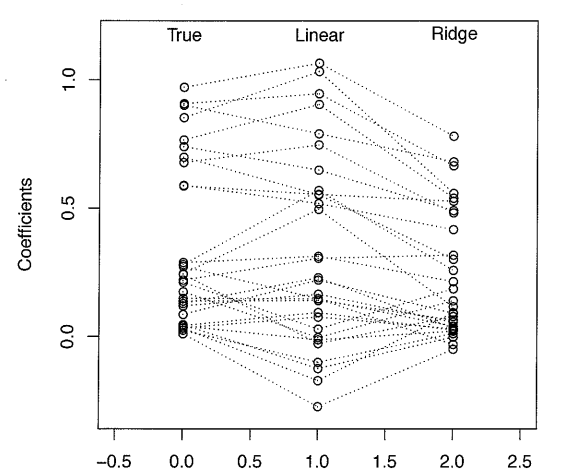
\includegraphics[width=0.5\linewidth]{img/shrinks}
\caption{Shrink of regression coefficients}
\label{fig:shrinks}
\end{figure}



On the other hand, the effect of adding the term $\lambda \mathbb{I}$
to the matrix $\mathbf{A}^\top \mathbf{A}$
(equation~(\ref{eq:optsolRR})) improves its condition number since it
increases its diagonal values when $\lambda > 0 $.  The matrix
$\mathbf{A}^\top \mathbf{A}$ is symmetrical ($(\mathbf{A}^\top
\mathbf{A})^\top = \mathbf{A}^\top \mathbf{A}$) and therefore
diagonalizable.  If we know the eigenvalue decomposition of $\mathbf{A}
= \mathbf{U\Sigma V^\top}$, then:

\begin{eqnarray*}
\mathbf{A}^\top \mathbf{A}+\lambda \mathbb{I}&=&\mathbf{V\Sigma^2
V}^\top + \lambda \mathbf{V} \mathbf{V}^\top\\ &=&\mathbf{V}
(\mathbf{\Sigma}^2+\lambda\mathbb{I}) \mathbf{V}^\top \, ,
\end{eqnarray*}

\noindent where

\begin{equation*}
\mathbf{\Sigma}^2+\lambda\mathbb{I}=
\begin{bmatrix}
\sigma^2_1 + \lambda & \, & \, \\
\, & \sigma^2_2 +\lambda & \, \\
\, & \, & \ddots & \, \\
\, & \, & \, & \sigma^2_n +\lambda \, .
\end{bmatrix}
\end{equation*}

where $\sigma_1 \geq \sigma_2 \geq \dots \geq \sigma_n$.

Since the condition number of a matrix $\mathbf{A}$ is defined as:

\begin{equation*}
	\kappa = \|\mathbf{A}\| \|\mathbf{A}^{-1}\|
\end{equation*}

If matrix $\mathbf{A}$ is non-singular, its condition number can be
expressed in terms of its singular values. The effect of adding the
regularization term affects the condition number as follows:

\begin{eqnarray*}
\kappa_{ols} &=& \|\mathbf{A}\| \|\mathbf{A}^{-1}\|=\frac{\sigma_1}{\sigma_n} \\
\kappa_{ridge} &=& \|\mathbf{A}^\intercal \mathbf{A} + \lambda \mathbb{I}\| 
\|(\mathbf{A}^\intercal \mathbf{A} + \lambda \mathbb{I})^{-1}\|=\frac{\sigma_1+\lambda}{\sigma_n + \lambda} \,
\end{eqnarray*}

It is easy to see that the term $\lambda$ improves the condition number: 

\begin{equation*}
        \frac{\sigma_1+\lambda}{\sigma_n + \lambda} <
        \frac{\sigma_1}{\sigma_n} \,  \qquad \forall \quad \lambda > 0
\end{equation*}


However, $\lambda$ cannot be too large. Tipically $\lambda$ is small and its
magnitude depends on the matrix $\mathbf{A}$.

For rank deficient matrices we know that $\text{det}(\mathbf{A A^\top})=0$, adding the
term $\lambda \mathbb{I}$ we have that $\text{det}(\mathbf{A A^\top}+\lambda \mathbb{I}) =
p(\lambda)$ where $p(\lambda)$ is a polynomial of degree $n$ ($\mathbf{A}$ is
$m \times n$). The zeros of $p(\lambda)$ are discretes, so it can be represented
as:

\[
p(\lambda) =
\lambda(\lambda-\lambda_1)^{n_1}(\lambda-\lambda_2)^{n_2}\dots(\lambda-\lambda_s)^{n_s}
\]

\noindent where $n_1 + n_2 + \dots + n_s = n$.

This means that $\lambda$ must be small in order to ensure that $p(\lambda)$
does not vanish.


\subsection{Selection of Lambda}

One of the ways to determine parameter $\lambda$ is using the bias-variance tradeoff (see section \ref{sec:biasvar}). This parameter is crucial for ridge regression since it could
reduce the expected prediction error by reducing variance, considering a biased
estimator. 
It is known that the prediction error can be express as a decomposition between bias and variance.

The solution of OLS is well known $\hat{\mathbf{X}}=(\mathbf{A}^\top \mathbf{A})^{-1}\mathbf{A}^\top \mathbf{Y}$, and its bias is:

\begin{eqnarray*}
Bias(\hat{f}(\hat{\mathbf{X}}) &=& E[\hat{\mathbf{X}}] - \mathbf{X} \\
&=& E[ (\mathbf{A}^\top \mathbf{A})^{-1}\mathbf{A}^\top \mathbf{Y}] - \mathbf{X} \\
&=& E[ (\mathbf{A}^\top \mathbf{A})^{-1}\mathbf{A}^\top (\mathbf{AX})] - \mathbf{X}  \\
&=& \mathbf{X}  - \mathbf{X}  \\
&=&  0
\end{eqnarray*}


The bias of ridge regression when $\mathbf{A A^\top}$ is non-singular
can be obtained expressing ridge regression solution
$\mathbf{\lambda}$ in terms of OLS solution $\hat{\mathbf{X}}$:

\begin{eqnarray*}
\mathbf{X}(\lambda) &=&( \mathbf{A}^\top \mathbf{A} + \lambda \mathbb{I})^{-1}\mathbf{A}^\top \mathbf{Y} \\
&=& (\mathbb{I} + \lambda (\mathbf{A}^\top \mathbf{A})^{-1})^{-1} (\mathbf{A}^\top \mathbf{A})^{-1}\mathbf{A}^\top \mathbf{Y} \\
&=&  (\mathbb{I} + \lambda (\mathbf{A}^\top \mathbf{A})^{-1})^{-1}  \hat{\mathbf{X}} \\
&=& \mathbf{W} \hat{\mathbf{X}} 
\end{eqnarray*}

\noindent where $\mathbf{W}  = (\mathbb{I} + \lambda (\mathbf{A}^\top
\mathbf{A})^{-1})^{-1}  $ it is defined for simplicity. Ridge
regression bias is then obtained as:

\begin{eqnarray*}
Bias(\mathbf{X}(\lambda)) &=& E[\mathbf{X}(\lambda)] - \mathbf{X} \\
&=& E[\mathbf{W}\hat{\mathbf{X}}] - \mathbf{X} \\
&=&  \mathbf{W} \mathbf{X} - \mathbf{X} \neq 0 
\end{eqnarray*}


The variance of OLS is:

\begin{equation*}
Var(\hat{\mathbf{X}}) = \sigma^2 (\mathbf{A}^\top \mathbf{A} )^{-1}
\end{equation*}

\noindent and the variance of ridge regression is:

\begin{eqnarray*}
Var(\mathbf{X}(\lambda)) &=& Var(\mathbf{W}\hat{\mathbf{X}}) \\
&=& E[(\mathbf{W}\hat{\mathbf{X}}-E[\mathbf{W}\hat{\mathbf{X}}])(\mathbf{W}\hat{\mathbf{X}}-E[\mathbf{W}\hat{\mathbf{X}}])^\top] \\
&=& \mathbf{W}E[(\hat{\mathbf{X}}-E[\hat{\mathbf{X}}])(\hat{\mathbf{X}}-E[\hat{\mathbf{X}}])^\top] \mathbf{W}^\top \\
&=& \mathbf{W}Var(\hat{\mathbf{X}})\mathbf{W}^\top \\
&=& \sigma^2 \mathbf{W}(\mathbf{A}^\top \mathbf{A} )^{-1}\mathbf{W}^\top
\end{eqnarray*}

\begin{figure}[h!]
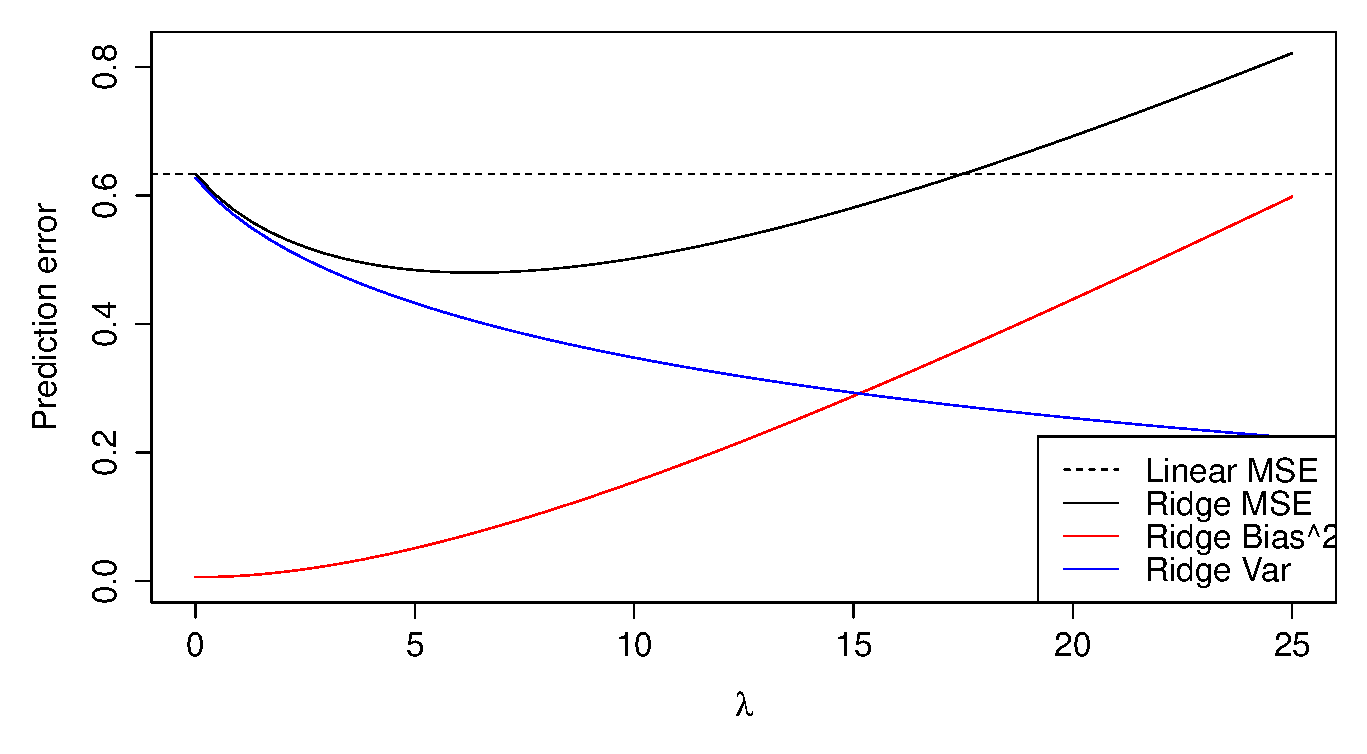
\includegraphics[width=\linewidth]{img/biasvariance}
\caption{Bias-variance tradeoff depending on lambda. Dotted line corresponds to OLS prediction error (invariant with lambda). Black line corresponds to RR prediction error which can be decomposed in $Bias^2$ (in red) + Variance (in blue).}
\label{fig:biasvariance}
\end{figure}	


The figure~\ref{fig:biasvariance} shows the bias-variance tradeoff
given by equation~(\ref{eq:bvtrade}). 

Despite OLS has zero bias,
its variance is greater than ridge for small values of $\lambda$.
It can be shown that, in terms of prediction error, ridge (black line)
is lower than OLS (dotted line)~\cite{hoerl1970}. Ridge regression shows an
increasing squared bias and a decreasing variance.

\textbf{Demo}\quad

Since $Bias(\mathbf{X}(\lambda)) \neq 0$ this imply that

\begin{equation*}
Bias(\mathbf{X}(\lambda)) ^2 > 0 
\end{equation*}

\noindent we know that $\mathbf{A}^\top
\mathbf{A}$ has an eigenvalue decomposition $\mathbf{A}^\top
\mathbf{A} = \mathbf{V} \Sigma \mathbf{V}^{-1}$.


\begin{eqnarray*}
Var(\mathbf{X}(\lambda)) &=& \sigma^2 \mathbf{W}(\mathbf{A}^\top \mathbf{A} )^{-1}\mathbf{W}^\top\\
Var(\mathbf{X}(\lambda)) &=& \sigma^2 (\mathbb{I} + \lambda (\mathbf{A}^\top
\mathbf{A})^{-1})^{-1} (\mathbf{A}^\top \mathbf{A} )^{-1}((\mathbb{I} + \lambda (\mathbf{A}^\top
\mathbf{A})^{-1})^{-1} )^\top \\
&=& \sigma^2 (\mathbb{I} + \lambda (\mathbf{V} \Sigma \mathbf{V}^{-1})^{-1} (\mathbf{V} \Sigma \mathbf{V}^{-1})^{-1}((\mathbb{I} + \lambda (\mathbf{V} \Sigma \mathbf{V}^{-1})^{-1})^{-1} )^\top \\
&=& \sigma^2 \mathbf{V} (\mathbb{I} + \lambda \Sigma^{-1})^{-1} \Sigma^{-1} (\mathbb{I} + \lambda \Sigma^{-1})^{-1}  \mathbf{V}^{-1}\\
&=& \sigma^2 \mathbf{V} \mathbf{D}^{-1} \mathbf{V}^{-1}
\end{eqnarray*}

\noindent where $\mathbf{D}^{-1}  = (\mathbb{I} + \lambda \Sigma^{-1})^{-1} \Sigma^{-1} (\mathbb{I} + \lambda \Sigma^{-1})^{-1}$ is a diagonal matrix with coefficients:

\begin{equation*}
d_i = \frac{\sigma_i^{-1}}{(1+\lambda\sigma_i^{-1})^2}
\end{equation*}

\subsection{Machine learning algorithms}
In recent years many successful machine learning applications have been developed. Artificial neural networks (ANN) and Support Vector Machines (SVM) have been some of the most popularly used machine learning algorithm \cite{haykin1998}. Historically, SVMs emerged after ANN.

The main characteristics of neural networks are that they have the ability to learn
complex nonlinear input-output relationships, they use sequential training procedures 
they adapt themselves to the data.

ANN is inspired by biological learning systems organised into layers and have unidirectional connections between the layers, feed-forward networks  (FFN) are the most used.  FFN consist of a series of layers. The first layer has a connection from the network input. Each subsequent layer has a connection from the previous layer. The final layer produces the network's output. Figure \ref{fig:ffn} shows a FFN with its different layers.

\begin{figure}[!h]
  \centering
  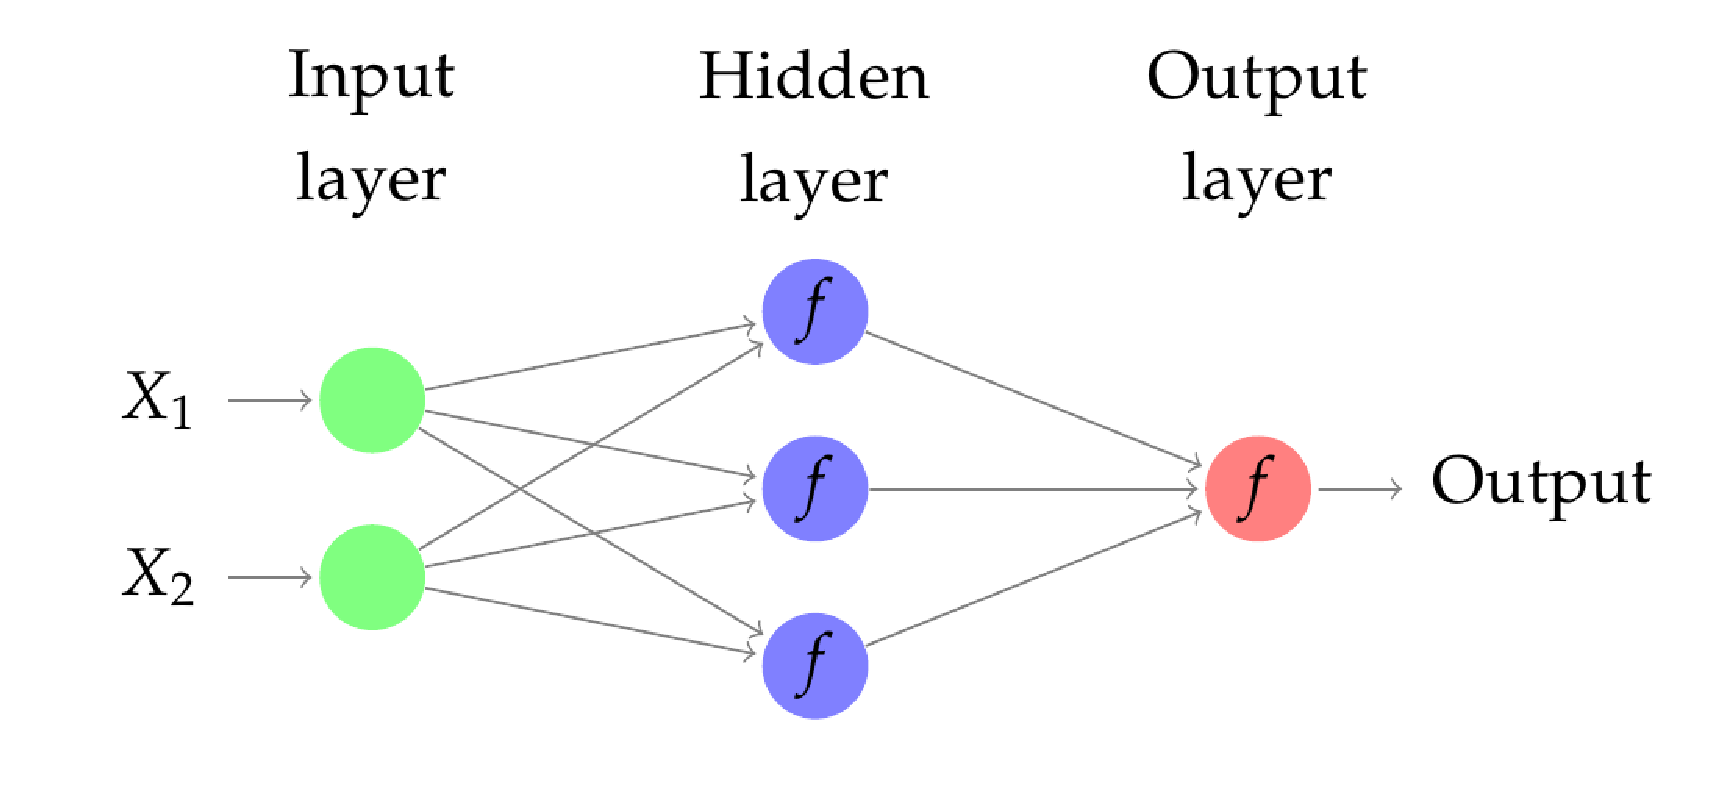
\includegraphics[width=0.8\textwidth]{img/ffn}
  \caption{Feed-forward neural network (FFN). FNN consists of an input layer, an output layer and at least one hidden layer between the input and output layer. }
  \label{fig:ffn}
\end{figure}


Support Vector Machine (SVM) was introduced in 1992 by Vapnik and his coworkers
\cite{boser1992}. In its original form, SVM is a training algorithm for linear classification. Only later it was used for regression, principal component analysis, novelty detection and also for non-linear case.  However, unlike ANN, it is very well 
based on theory in statistical learning \cite{cortes1995}.  SVM tunes the capacity of 
maximising the margin between the training patterns and the decision boundary. The
solution is expressed as a linear combination of supporting patterns, which are the training patterns close to the decision boundary, called the support vectors.

The major difference between SVM and ANN is in the error optimisation. In ANN, the aim of learning is to obtain a set of weight values which minimise the training error 
minimum while training adjust the capacity of the machine. 

For nonlinear case, SVM mapped the data sets of input space into a higher dimensional feature space, which is linear and the large margin learning algorithm is then applied. However, the mapping can be implicitly done by kernel functions. In the high dimensional feature space, simpler and linear hyper plane classifiers that have maximal margin between the classes can be obtained.

%\subsection{Kernel methods}
%Kernel functions may be used to introduce a nonlinear separation
%in input space despite the linear classifier in decision space
\newpage
\section{Online learning} \label{sec:onoffline}

Online learning is a supervised machine learning framework that is useful when
we have sequential access to a sample only once.  This differs from the
classical batch learning, where there is an entire data set available and the
learner can build the internal model without any limits in accessing the data.
In batch learning, there is time enough to carefully analyse the dataset, build
large predictive models and combine them in a sophisticated way. However, when
execution time is critical and new data is required to be included in the model,
online learning algorithms are a better option.

In batch learning, the training phase is commonly a computationally expensive
process. Therefore, when new data arrives it can't be included easily to the
model. Moreover, it could happen that we won't have enough time to process the
new data before more data arrives. In online learning algorithms there is no
training phase, but the model is updated and evaluated at every time step. This
model updating is computationally less expensive than a training phase.
Online algorithms allow incremental learning by processing one instance at a
time. This is done updating the current model instead of building the model from
scratch.

Online learning is also useful when some past data may be irrelevant
or we want to improve computational efficiency. However, the use of less
historical data could affect accuracy.

The goal of online learning is the same as batch learning, predicting targets as
accurate as possible. For example, stock market prediction can be seen as online
learning. The algorithm makes a prediction of the stock, little time after the
real stock price is available, this information can be incorporated to the
learner to further improve the prediction accuracy. In general, there is too
much data available in an online learning setup, the data set grows
continuously. Offline learning has equal or superior accuracy compared to online
learning when the same amount of data is used.

Classic statistical theory of sequential prediction enforces strong assumptions
on the statistical properties of the input sequence (for example, stationary
stochastic process). However, these assumptions can be unknown or change over
time. In online learning there is no previous assumption about the data and the
sequence is allowed to be deterministic, stochastic or even adaptive.  

Moreover, in case we receive data streams, ANN or SVM cannot introduce new
information into the model without a re-training process, so we will have to use
the same non-updated model until we decide to compute another one if it is
possible.  Online learning algorithms allow one example at a time to be
introduced into an existing model incrementally \cite{vovk2005}. This is
extremely important when the problem has large data streams and real-time
forecasting must be done.  This is the most common scenario when we want to
forecast a wide range of data such as stock prices and volatilities, electricity
power, intrusion detection, web-mining, server load, etc.  Besides, many
problems of high interest in machine learning can be treated as online ones and
they can also use these types of algorithms.

The online learning framework was first introduced in the perceptron algorithm
\cite{rosenblatt58}. There are several other widely used online methods such as
passive-aggressive \cite{crammerETall2006}, stochastic gradient descent
\cite{zhang2004}, aggregating algorithm \cite{vovk2001} and the second order
perceptron \cite{cesa-bianchi2005}.  In \cite{cesa-bianchi2006} an in-depth
analysis of online learning is provided.

The motivation for online learning is to obtain computational efficiency and
tackle the shifting problem, i.e. that the distribution of the data is unknown
or changes over time. Online learning algorithms can deal with this problem
because they have a tracking ability which is a strategy based on retaining weak
dependence on past examples by using two types of models: 

\textit{a)} \textbf{memory boundedness:} consists of limiting the number of
support vectors in order to improve computational efficiency. One example of
this is the budget perceptron~\cite{crammeretal2004} which reduces the number of
examples used for prediction. Alternatively, in the forgetron
algorithm~\cite{dekeletal2008} the damage caused by removing old examples is
discussed, which can be avoided by removing samples with small influences. Other
examples are the sliding window kernel (RLS)~\cite{vanvaerenberghetal2006},
which only considers a sliding window of the most recent data, and in
\cite{arce+salinas2012} is shown a variant of aggregating algorithm for
regression~\cite{vovk2001} considering only a sliding window of the most recent
data, optimising also common matrix operations.

\textit{b)} \textbf{weight decay:} one example of this is the shifting
perceptron algorithm which implements an exponential decaying scheme for the
examples~\cite{cavallantietal2007}.  Performance of an online learning algorithm
is measured by the cumulative loss it suffers along its run on a sequence of
examples. In order to minimise this loss, the learner may update the hypothesis
after each round so as to be more accurate in later rounds.


There is sometimes confusion about online and incremental learning concepts.
Incremental learning refers to any online learning process that learns the same
model as would be learnt by a batch learning algorithm. 

Incremental learning is useful when the input to a learning process is stream
data, with the need or desire to be able to use the result of learning at any
point in time, based on the input observations received so far. 

Incremental learning is very useful when there is no need to record fundamental
data and only a summary needs to be retained. Due to this, incremental
algorithms are often characterised as memoryless, because no memory of past data
is required.  The algorithm is online but not incremental if it doesn't produce
the same result for all observations that the corresponding batch algorithm
would for these same observations.

Algorithm~\ref{alg:onlinealg} shows the online learning algorithm structure:

\begin{algorithm}[ht]
\begin{algorithmic}[1]
    \STATE Receives input $\mathbf{x}_t$
    \STATE Makes prediction $\mathbf{\hat{y}}_t$
    \STATE Receives response $\mathbf{y}_t$
    \STATE Incurs loss $l_t(\mathbf{y}_t,\mathbf{\hat{y}}_t)$
\end{algorithmic}
\caption{Structure of a Learning System}
\label{alg:onlinealg}
\end{algorithm}

\noindent where $l$ is some loss function. Performance is later measured after
$T$ trials as:

\begin{equation*}
L_T = \sum_{t=1}^T l_t(\mathbf{y}_t,\mathbf{\hat{y}}_t)
\end{equation*}

The objective is minimize this loss function for all instances.
The quality of online learning algorithms is measured by a quantity known as
regret which is the difference between the performance of the online algorithm
and its optimal predictor $E^* \in \Theta$ given by:

\begin{equation*}
L^*_T= \text{min}_{E \in \Theta} L_T^E \, ,
\end{equation*}

\noindent where $L_T^E = \sum_{t=1}^T
l_t(\mathbf{y}_t,\mathbf{y}^E_t)$ and $\mathbf{y}^E_t$ is the expert estimation. 

Therefore regret is defined as:

\begin{equation*}
R_T = L_T - L^*_T
\end{equation*}

\subsection{Competitive analysis}

Competitive analysis was designed for analysing the performance of an online algorithm compared with its optimal offline algorithm. An optimal offline algorithm can view the sequences of requests in advance. The effectiveness of an online algorithm \cite{sleator1985} may be measured by its competitive ratio which is the worst-case ratio of the online algorithm and the optimal offline algorithm.



\subsection{Online Ridge Regression}

Online RR is the online formulation of the regularised Least Squares method
and is based on the following equivalent formulation of the RR optimal solution.

Since 
\begin{equation}
\label{eq:notation}
	\mathbf{A} = 
\left[
  \begin{tabular}{c>{$}c<{$}c}
    --- & \mathbf{a}^{\top}_{1} & ---\\
    --- & \mathbf{a}^{\top}_{2} & ---\\
    & \vdots & \\
    --- & \mathbf{a}^{\top}_{m} & ---
  \end{tabular}
\right]
\quad \text{and} \quad
\mathbf{B} =
\left[
  \begin{tabular}{c>{$}c<{$}c}
    --- & \mathbf{b}_{1} & ---\\
    --- & \mathbf{b}_{2} & ---\\
    & \vdots & \\
    --- & \mathbf{b}_{m} & ---
  \end{tabular}
\right]
\end{equation}

Equation~(\ref{eq:optsolRR}) can also be written as:
\begin{eqnarray*}
\label{eq:RReapand}
\mathbf{\mathbf{X}}_{\text{ridge}}&=&(\mathbf{A}^\top \mathbf{A}+ \lambda
\mathbb{I})^{-1}\mathbf{A}^\top \mathbf{Y} \\
&=& \displaystyle \big (\sum_{t=1}^m
\mathbf{a}_t \mathbf{a}_t  ^\top + \lambda \mathbb{I}\big )^{-1}
\sum_{t=1}^m \mathbf{a}_t \mathbf{y}_t \, .
\end{eqnarray*}

Lets define $\displaystyle\mathbf{S}= \sum_{t=1}^m \mathbf{a}_t
\mathbf{a}_t  ^\top + \lambda \mathbb{I} $ and $\mathbf{W}=
\displaystyle\sum_{t=1}^m \mathbf{a}_t \mathbf{y}_t$, so the
algorithm~\ref{alg:RR} shows the iterative formulation:

\begin{algorithm}[H]
\begin{algorithmic}[1]
\REQUIRE $\,$ \\
$\{\mathbf{a}_1,\dots,\mathbf{a}_{m} \}$: $m$ input vectors \\
$\{\mathbf{y}_1,\dots,\mathbf{y}_{m} \}$: $m$ target vectors \\
$\lambda$: regularization parameter \\
\ENSURE  $\,$ \\
$\{f(\mathbf{a}_1),\dots,f(\mathbf{a}_{m}) \}$: model predictions \\
\STATE Initialize $\mathbf{S}=\lambda \mathbb{I}$
and $\mathbf{W}=0$
\FOR { $t = 1$ to $m$ }
	\STATE read new $\mathbf{a}_t$
	\STATE $\mathbf{X}=\mathbf{S}^{-1}\mathbf{W}$
	\STATE output prediction $f(\mathbf{a}_t) = \mathbf{X}^\top \mathbf{a}_t$
   	\STATE $\mathbf{S} = \mathbf{S} + \mathbf{a}_t \mathbf{a}_t^\top$
   	\STATE Read new $y_t$
    	\STATE $\mathbf{W} = \mathbf{W} + \mathbf{a}_t \mathbf{y}_t$
\ENDFOR
\end{algorithmic}
\caption{Online Ridge Regression}
\label{alg:RR}
\end{algorithm}



\subsection{The Aggregating Algorithm for Regression}

The AAR, proposed by~\cite{vovk2001} (also known as Vovk-Azoury-Warmuth predictor ~\cite{azoury2001}), is an application of the aggregating
algorithm to the problem of regression. The idea is introduce the new input
vector $\mathbf{x}_{m+1}$ to solve the model parameters: 

\begin{equation}
\label{eq:AARexpand}
\mathbf{X}_{aar} = \displaystyle \big (\sum_{t=1}^{m+1}
\mathbf{a}_t \mathbf{a}_t  ^\intercal + \gamma \mathbb{I}\big )^{-1}
\sum_{t=1}^m \mathbf{a}_t \mathbf{y}_t \, .
\end{equation}

If we define $\displaystyle\mathbf{S}= \sum_{t=1}^{m+1} \mathbf{a}_t
\mathbf{a}_t  ^\intercal + \gamma \mathbb{I} $ and $\mathbf{W}=
\displaystyle\sum_{t=1}^m \mathbf{a}_t \mathbf{y}_t$, the
algorithm~\ref{alg:AAR} is slightly different to the algorithm~\ref{alg:RR}, 
which updated matrix $\mathbf{S}$ before making the prediction:

\begin{algorithm}[ht]
\begin{algorithmic}[1]
\REQUIRE $\,$ \\
$\{\mathbf{a}_1,\dots,\mathbf{a}_{m} \}$: $m$ input vectors \\
$\{\mathbf{y}_1,\dots,\mathbf{y}_{m} \}$: $m$ target vectors \\
$\lambda$: regularisation parameter \\
\ENSURE  $\,$ \\
$\{f(\mathbf{a}_1),\dots,f(\mathbf{a}_{m}) \}$: model predictions \\
\STATE Initialize $\mathbf{S}=\lambda \mathbb{I}$
and $\mathbf{W}=0$
\FOR { $t = 1$ to $m$ }
	\STATE read new $\mathbf{a}_t$
   	\STATE $\mathbf{S} = \mathbf{S} + \mathbf{a}_t \mathbf{a}_t^\intercal$
	\STATE $\mathbf{X}=\mathbf{S}^{-1}\mathbf{W}$
	\STATE output prediction $f(\mathbf{a}_t) = \mathbf{X}^\intercal \mathbf{a}_t$
   	\STATE Read new $\mathbf{y}_t$
    	\STATE $\mathbf{W} = \mathbf{W} + \mathbf{a}_t \mathbf{y}_t$
\ENDFOR
\end{algorithmic}
\caption{{\em The aggregating algorithm for regression}}
\label{alg:AAR}
\end{algorithm}


\subsection{Efficient computation}
In regression problems we always require getting a matrix inverse which is
computationally expensive. However, in stream data problems there is a way to
obtain a matrix inverse approximation using the Sherman-Morrison-Woodbury. This
formula allows to get the inverse of a matrix $\mathbf{A+uv^\top}$ if we previously calculated the
inverse of $\mathbf{A}$ as follows:

\begin{equation}
\label{eq:SMW}
(\mathbf{A+uv^\top})^{-1}=\mathbf{A}^{-1}-
\frac{\mathbf{A^{-1}uv^\top A^{-1}}}{\mathbf{1+v^\top A^{-1}u}}
\end{equation}


Alternatively, Coleman and
Sun~\cite{coleman+sun2010} presented an iterative algorithm which
uses $\mathbf{X}(\lambda)$ to approximate $\mathbf{X}(0)$.


Using the compact SVD (shown in equation~(\ref{eq:compactsvd}))
$\mathbf{X}(\lambda)$ is expressed as follows:


\begin{eqnarray}
\label{eq:optsolRRsvd}
\mathbf{X}(\lambda) & = & (\mathbf{A}^\top \mathbf{A}+ \lambda
\mathbb{I})^{-1}\mathbf{A}^\top \mathbf{Y} \nonumber \\
& = &\mathbf{V}_1(\Sigma_1^2+\lambda \mathbb{I})^{-1}\mathbf{\Sigma_1
U_1^\top Y}
\end{eqnarray}

\noindent where is easy to see that $\mathbf{X}(\lambda) \rightarrow
\mathbf{\hat{X}}=\mathbf{V}_1 \mathbf{\Sigma}_1^{-1}\mathbf{U}_1^\top
\mathbf{Y}$ as $\lambda \rightarrow 0$. 

The method consists in obtaining $\mathbf{X}(\lambda)$ and then refine
by adding more terms of its Taylor expansion to approximate
$\mathbf{X}(0) = \mathbf{\hat{X}}$. The Taylor expansion about $\lambda_0$ is:

\begin{equation}
\label{eq:taylor}
    \mathbf{X}(\lambda)=\mathbf{X}(\lambda_0) + \sum_{k=1}^\infty
    \mathbf{s}_k(\lambda-\lambda_0)^{k}
\end{equation}


\noindent where $\mathbf{s}_k=\frac{1}{k!}\mathbf{X}(\lambda)^{(k)}$
and $\mathbf{X}(\lambda)^{(k)}$ is obtained by taking differences 
$\frac{\partial}{\partial \lambda}$ of:  

\begin{eqnarray*}
(\mathbf{A}^\top \mathbf{A}+ \lambda\mathbb{I}) \mathbf{X}(\lambda) & = & \mathbf{A}^\top \mathbf{Y}\\
(\mathbf{A}^\top \mathbf{A}+ \lambda\mathbb{I}) \mathbf{X}(\lambda)^{(1)} + \mathbf{X}(\lambda)& = & 0 \\
\mathbf{X}(\lambda)^{(1)}  &=& -(\mathbf{A}^\top \mathbf{A}+ \lambda\mathbb{I}) ^{-1} \mathbf{X}(\lambda) \\
\mathbf{X}(\lambda)^{(2)}  &=& -2(\mathbf{A}^\top \mathbf{A}+ \lambda\mathbb{I}) ^{-1} \mathbf{X}(\lambda)^{(1)} \\
& \vdots & \\
\mathbf{X}(\lambda)^{(k)}  &=& -k(\mathbf{A}^\top \mathbf{A}+ \lambda\mathbb{I}) ^{-1} \mathbf{X}(\lambda)^{(k-1)} 
\end{eqnarray*}



\noindent for $\lambda=0$ we have:

\begin{equation}
\label{eq:taylor}
    \mathbf{X}(0)=\mathbf{X}(\lambda_0) + \sum_{k=1}^\infty
     (-1)^k \mathbf{s}_k \lambda_0^k
\end{equation}


\noindent therefore in order to ensure convergence, we can see that$\lambda_0$
selection cannot be large. 

The algorithm for computing $\mathbf{X}(0)$ is the following:

\begin{algorithm}[H]
\begin{algorithmic}[1]
\REQUIRE $\,$ \\
$\mathbf{A}$: design matrix \\
$\mathbf{Y}$: response matrix \\
$\lambda$: rank deficient parameter \\
\ENSURE  $\,$ \\
$\mathbf{X}$: parameters \\
\STATE $\mathbf{M}=\mathbf{A^\top A}$ \\
\STATE Initialize $\mathbf{Q R}=\mathbf{M}$ \\
\STATE $\mathbf{X} = \mathbf{R^{-1}Q^\top Y}$ \\
\STATE $\mathbf{s} = \mathbf{X}$ \\
\FOR { $i = 1,2,3,\dots$ }
	\STATE $\mathbf{s} =
        -(\mathbf{M}+\lambda\mathbb{I})^{-1}\mathbf{s}$\\
	\STATE $\mathbf{X}=\mathbf{X} + (-1)^i {\color{red}\mathbf{s}
        \lambda^i}$
\ENDFOR
\end{algorithmic}
\caption{Algorithm for handling rank deficient matrices}
\label{alg:coleman}
\end{algorithm}

The algorithm~\ref{alg:coleman} solves equation~(\ref{eq:taylor}). However, this
version is unstable since typically $\|\mathbf{s}\|$ is very large and
$\lambda^i$ is very small ($\lambda$ is small).

The following algorithm shows a more stable version of
algorithm~\ref{alg:coleman}.


\begin{algorithm}[H]
\begin{algorithmic}[1]
\REQUIRE $\,$ \\
$\mathbf{A}$: design matrix \\
$\mathbf{Y}$: response matrix \\
$\lambda$: rank deficient parameter \\
\ENSURE  $\,$ \\
$\mathbf{X}$: parameters \\
\STATE $\mathbf{M}=\mathbf{A^\top A}$ \\
\STATE Initialize $\mathbf{Q R}=\mathbf{M}$ \\
\STATE $\mathbf{X} = \mathbf{R^{-1}Q^\top Y}$ \\
\STATE $\mathbf{t} = \mathbf{X}$ \\
\FOR { $i = 1,2,3,\dots$ }
        \STATE $\mathbf{t} =\lambda \mathbf{t}$  
        \STATE $\mathbf{t} =  -(\mathbf{M}+\lambda\mathbb{I})^{-1}\mathbf{t}$
	\STATE $\mathbf{X}=\mathbf{X} + \mathbf{t}$
\ENDFOR
\end{algorithmic}
\caption{Algorithm for handling rank deficient matrices improved}
\label{alg:colemanimproved}
\end{algorithm}

Both algorithms are equivalent, but algorithm~\ref{alg:colemanimproved} is more
stable and converges in typically less than 10 steps.
It is important to notice that the QR factorisation is computed only once and it
is computationally less expensive than the SVD.


Despite the bias-variance tradeoff provides a conceptual framework for
determining a good model, is not directly useful. Some popular methods
for determine model selection are:

\begin{itemize}
    \item Akaike information criterion (AIC) (Akaike, 1974)
    \item Bootstrap-based selection (Efron and Tibshirani, 1997)
    \item Cross-validation (Stone, 1974)
\end{itemize}

On the other hand, $\lambda$ can also be used to reduce computational time as it
is shown in equation~(\ref{eq:taylor}). Golub (~\cite{golub1965}) suggested that
$\lambda$ be chosen so that:

\[
\frac{\lambda}{\lambda + \delta^2} < 0.1
\]

\noindent where $\delta$ is a lower bound of the smallest non-zero singular
value $\sigma_k$. One approach is to choose the greatest lower bound for
$\delta=\sigma_k$. Hence:

\[
\frac{\lambda}{\lambda + \sigma_k^2} < 0.1
\]

\noindent if we choose $\lambda=\beta \sigma_k^2$ then we get the following
relation:


\[
\frac{\beta \sigma_k^2}{\beta \sigma_k^2 + \sigma_k^2} =
\frac{\beta}{\beta+1} < 0.1 \Rightarrow \beta < \frac{1}{9}  
\]

Experiments done by ~\cite{coleman+sun2010} have shown that $\beta = 0.01$
produces satisfactory results. This means that $\lambda = 0.01 \sigma_k^2$.

However, get $\sigma_k$ imply obtaining first the SVD, which is
computational expensive.

Since the algorithm presented by ~\cite{coleman+sun2010} already compute the QR
factorization of the matrix $\mathbf{A}$ they show a procedure for getting
a $\lambda$ approximation using QR.

\begin{enumerate}
\item Compute QR factorization: $\mathbf{A} = \mathbf{Q_1R_1}$
\item Let $\mathbf{W}$ denote the set of absolute values of the nonzero diagonal
elements of $\mathbf{R_1}$. Let $w_{\text{min}}$ and $w_{\text{max}}$ denote the
smallest and largest elements of $\mathbf{W}$ respectively. Both 
$\lambda_1 = \hat{\beta} w_{\text{min}}^2$
$\lambda_2 = \hat{\beta} \frac{w_{\text{min}}^2}{w_{\text{max}}^2}$ where
$\hat{\beta}=0.00025$ produce satisfactory results.
\item The $\lambda_{\text{QR}}$ approximation is obtained as:
$\lambda_{\text{QR}} = \frac{\lambda_1 + \lambda_2}{2}$  
\end{enumerate}

\newpage

\section{Evaluation methods} \label{sec:evaluation}

Forecast performance is evaluated using different methods. We have chosen three
measures usually used:
\begin{description}
\item[MAPE] Mean Average Percent Error which presents forecast errors as a
percentage.
\begin{equation}\label{eq:MAPE}
\text{MAPE} = \frac{1}{N} \sum_{t=1}^{N} 
\frac{\left|\mathbf{y}_t-\hat{\mathbf{y}}_t\right|}{\left|\mathbf{y}_t\right|}
 \times 100 
\end{equation}
\item[MAE] Mean Average Error which measures the distance between forecasts to the
true value.
\begin{equation}\label{eq:MAE}
\text{MAE} = \frac{1}{N} \sum_{t=1}^{N} 
\left| 
\mathbf{y}_t-\hat{\mathbf{y}}_t
\right| 
\end{equation}
\item[MSE]  Mean Square Error measures the distance between forecasts
and the true values and large deviations from the true value have a
large impact due to squaring forecast error.
\begin{equation}\label{eq:MSE}
\text{MSE} = 
\frac{\displaystyle \sum_{t=1}^{N} (\mathbf{y}_t-\hat{\mathbf{y}}_t)^2}{N}
\end{equation}
\item[RMSE] Root Mean Square Error also measures the distance between forecasts
to the true values but, unlike MAE, large deviations from the true value have a
large impact on RMSE due to squaring forecast error.
\begin{equation}\label{eq:RMSE}
\text{RMSE} = \sqrt{
\frac{\displaystyle \sum_{t=1}^{N} (\mathbf{y}_t-\hat{\mathbf{y}}_t)^2}{N}}
\end{equation}
\item[$U$-statistic] the Theil's $U$-statistic, presented by
\cite{theil1966}, is a unit free measure obtained as the ratio between the root
MSE (RMSE) of a model and the RMSE of the naive random walk model. A
$U$-statistic less than 1 implies the performance is better than the naive
model.
\end{description}


\section{Model selection} \label{sec:pselection}
Akaike Information Criterion (AIC) is often used in model selection where AIC
with smaller values are preferred since they represent a trade-off between bias
and variance.  AIC is obtained as follows:

\begin{equation}
\label{eq:aicformula}
AIC = \underset{\text{bias}}{-\frac{2l}{N}} + 
\underset{\text{variance}}{\frac{2k}{N}}
\end{equation}

\noindent where 

\begin{description}
\item[l] is the loglikelihood function
\item[k] number of estimated parameters
\item[N] number of observations
\end{description}

Loglikelihood function is obtained from the Residual Sum of Squares (RSS):

\begin{equation}
\label{eq:ll}
l = -\frac{N}{2} \left(1 + ln(2\pi) + ln\left(\frac{RSS}{N}\right)\right) 
\end{equation}
